\documentclass{article}
\usepackage{amsmath}
\usepackage{graphicx}
\usepackage{hyperref}
\usepackage[margin=1in]{geometry}
\usepackage{placeins} % For \FloatBarrier

\title{Homework Number: Seven\\ \large Monetary Policy 1: Money, the Fed, and Implementation}
\author{Team Two}
\date{July 6th, 2024}

\begin{document}

\maketitle

\section{Money}

\subsection{The Problem of the Double Coincidence of Wants}
The ``problem of the double coincidence of wants'' refers to the difficulty in barter systems where two parties each desire exactly what the other has to offer at the same time. This problem could entail many transactions before the good was finally received, creating a complex and inefficient loop. Money solves this problem by acting as a medium of exchange that is universally accepted, thus eliminating the need for both parties to want each other's goods or services simultaneously. 

\textbf{Example:} In the absence of money, if a baker wants to trade bread for a farmer's eggs, but the farmer does not need bread, the trade cannot happen unless they find a third party who wants bread and has something the farmer wants. This loop can continue until a suitable trade is found, causing significant inefficiency.

\noindent\rule{\linewidth}{0.5pt}

\subsection{Can Something Be ``Money'' if it is Not Widely Accepted?}
For something to function as money, it must be widely accepted as a medium of exchange, a unit of account, and a store of value. If it is not widely accepted, it cannot serve these purposes effectively. 

\textbf{Example:} If a local community agrees to use a unique token for transactions, it can act as money within that community, but it would not be considered money outside of it. Hence, broad acceptance is crucial.

\noindent\rule{\linewidth}{0.5pt}

\subsection{Challenging the Statement: ``There Cannot Be Inflation Without Money''}
The statement that ``there cannot be inflation without money'' is true. Without money, only specific goods could increase in price, not the general price level of goods and services. Inflation refers to a general rise in prices across the economy, which requires a medium of exchange like money. In a barter economy, certain goods might become more valuable, but this does not constitute inflation as understood in a monetary economy.

\noindent\rule{\linewidth}{0.5pt}

\subsection{Monetary Policy in the Absence of Money}
Monetary policy is designed to manage the supply of money and interest rates to influence economic activity. Without money, the mechanisms for such policies would not exist as barter systems do not use money. Therefore, in the absence of money, there would be no need for monetary policy.

\noindent\rule{\linewidth}{1pt}

\section{The Federal Reserve}

\subsection{Reasons for the Creation of the Fed}
The Federal Reserve was created to provide the United States with a safer, more flexible, and more stable monetary and financial system. The primary motivations included addressing bank panics, managing inflation, and stabilizing the economy.

\noindent\rule{\linewidth}{0.5pt}

\subsection{Legal Document Supporting the Fed}
The Federal Reserve Act is the legal document that supports the Fed's existence. It was signed into law on December 23, 1913. Historical episodes involved include the Panic of 1907, which highlighted the need for central banking reforms, and extensive debates and negotiations in Congress about the structure and control of the proposed central bank. Another important episode was the Aldrich-Vreeland Act of 1908, which created the National Monetary Commission, whose reports were essential to the creation of the Fed.

\noindent\rule{\linewidth}{0.5pt}

\subsection{Components of the Federal Reserve System}
The three components are:
\begin{enumerate}
    \item The Board of Governors
    \item The Federal Open Market Committee (FOMC)
    \item The 12 Regional Federal Reserve Banks
\end{enumerate}
The FOMC was not part of the original creation; it was established later to oversee open market operations.

\noindent\rule{\linewidth}{0.5pt}

\subsection{Functions of the Fed}
\begin{enumerate}
    \item Conducting national monetary policy
    \item Supervising and regulating banks
    \item Maintaining financial system stability
    \item Providing financial services to the U.S. government, financial institutions, and the public
\end{enumerate}

\noindent\rule{\linewidth}{0.5pt}

\subsection{Ownership of the Fed}
The Federal Reserve Banks are owned by private member banks, which hold stock in their respective regional Federal Reserve Bank.

\noindent\rule{\linewidth}{0.5pt}

\subsection{Funding of the Fed}
The Fed finances itself through interest on government securities, fees for services provided to financial institutions, and income from foreign currency investments. It also earns interest on loans it makes to banks, such as when banks need to meet reserve requirements. The Fed does not rely on congressional appropriations.

\noindent\rule{\linewidth}{0.5pt}

\subsection{Regional Fed Banks and Presidents}
There are 12 regional Federal Reserve Banks located in:
\begin{itemize}
    \item Boston: Susan M. Collins
    \item New York: John C. Williams
    \item Philadelphia: Patrick T. Harker
    \item Cleveland: Mark S. Meder (Interim President)
    \item Richmond: Tom Barkin
    \item Atlanta: Raphael Bostic
    \item Chicago: Austan D. Goolsbee
    \item St.\ Louis: Alberto G. Musalem
    \item Minneapolis: Neel Kashkari
    \item Kansas City: Jeffrey R. Schmid
    \item Dallas: Lorie K. Logan
    \item San Francisco: Mary C. Daly
\end{itemize}
The presidents of each regional Fed are appointed by their respective bank's board of directors, subject to approval by the Board of Governors.

\noindent\rule{\linewidth}{0.5pt}

\subsection{Board of Governors}
The Board of Governors currently has seven members appointed by the President of the United States and confirmed by the Senate. Each member serves a staggered 14-year term, meaning one term begins every two years on February 1 of even-numbered years. A member who serves a full term may not be reappointed. A member who completes an unexpired portion of a term may be reappointed. All terms end on their statutory date regardless of the date on which the member is sworn into office. The current members are:
\begin{itemize}
    \item Jerome H. Powell (Chair)
    \item Michael S. Barr (Vice Chair for Supervision)
    \item Philip N. Jefferson (Vice Chair)
    \item Michelle W. Bowman
    \item Lisa D. Cook
    \item Adriana D. Kugler
    \item Christopher J. Waller
\end{itemize}

\noindent\rule{\linewidth}{0.5pt}

\subsection{Chair and Vice Chairs of the Fed}
The current Chair of the Fed is Jerome Powell. The current Vice Chair is Philip N. Jefferson. Michael S. Barr is the current Vice Chair for Supervision. The Chair and Vice Chair of the Fed are appointed by the President of the United States from among the sitting Governors and confirmed by the Senate. The Chair serves a four-year term and can be reappointed.

\noindent\rule{\linewidth}{0.5pt}

\subsection{Federal Open Market Committee (FOMC)}
The FOMC consists of the seven members of the Board of Governors and five Reserve Bank presidents. They meet eight times a year to discuss and set monetary policy. The Beige Book is a report published before each meeting, summarizing economic conditions across the districts, which the FOMC uses to inform their decisions. The current members are:
\begin{itemize}
    \item Jerome H. Powell (Chair)
    \item John C. Williams (Vice Chair)
    \item Michael S. Barr
    \item Michelle W. Bowman
    \item Lisa D. Cook
    \item Philip N. Jefferson
    \item Adriana D. Kugler
    \item Christopher J. Waller
    \item Tom Barkin
    \item Raphael Bostic
    \item Mary C. Daly
    \item Patrick T. Harker
    \item Neel Kashkari
    \item Lorie K. Logan
    \item Mark S. Meder
    \item Alberto G. Musalem
    \item Jeffrey R. Schmid
\end{itemize}

\noindent\rule{\linewidth}{0.5pt}

\subsection{Tools of the Fed’s Monetary Policy}
\begin{enumerate}
    \item \textbf{Open Market Operations (OMO):} The buying and selling of government securities to influence the money supply and interest rates.
    \item \textbf{Discount Rate:} The interest rate charged to commercial banks and other financial institutions for short-term loans from the Federal Reserve Bank.
    \item \textbf{Reserve Requirements:} The amount of funds that a depository institution must hold in reserve against specified deposit liabilities.
    \item \textbf{Interest on Reserves (IOR):} The rate paid on excess reserves that banks hold at the Fed.
    \item \textbf{Forward Guidance:} The communication by the Fed regarding the future path of monetary policy.
\end{enumerate}

\noindent\rule{\linewidth}{0.5pt}

\subsection{Announcing Monetary Policy Decisions}
The Fed announces its monetary policy decisions through press releases, post-meeting statements, and press conferences. The decision regarding the federal funds rate target is usually a band (range of numbers).

\noindent\rule{\linewidth}{1pt}

\section{Implementation of Monetary Policy}

\subsection{Influencing Interest Rates}
The central bank does not directly control the real interest rate but influences it through monetary policy tools that affect inflation expectations and nominal rates. The central bank can directly influence the one-year nominal interest rate through open market operations and setting the discount rate. To manipulate aggregate demand, a central bank influences the real interest rate by controlling the very short-term nominal interest rate and announcing the path of future short-term policy rates. This approach works if the term premium is stable and the path of short-term rates is predictable.

\noindent\rule{\linewidth}{0.5pt}

\subsection{Term Structure of Interest Rates}
The ``term structure of interest rates'' refers to the relationship between interest rates (or bond yields) and different terms to maturity. It is often depicted as a yield curve, which shows the yields on bonds of varying maturities at a specific point in time. Maturity refers to when the instrument will pay back the principal.
\begin{figure}[ht!]
    \centering
    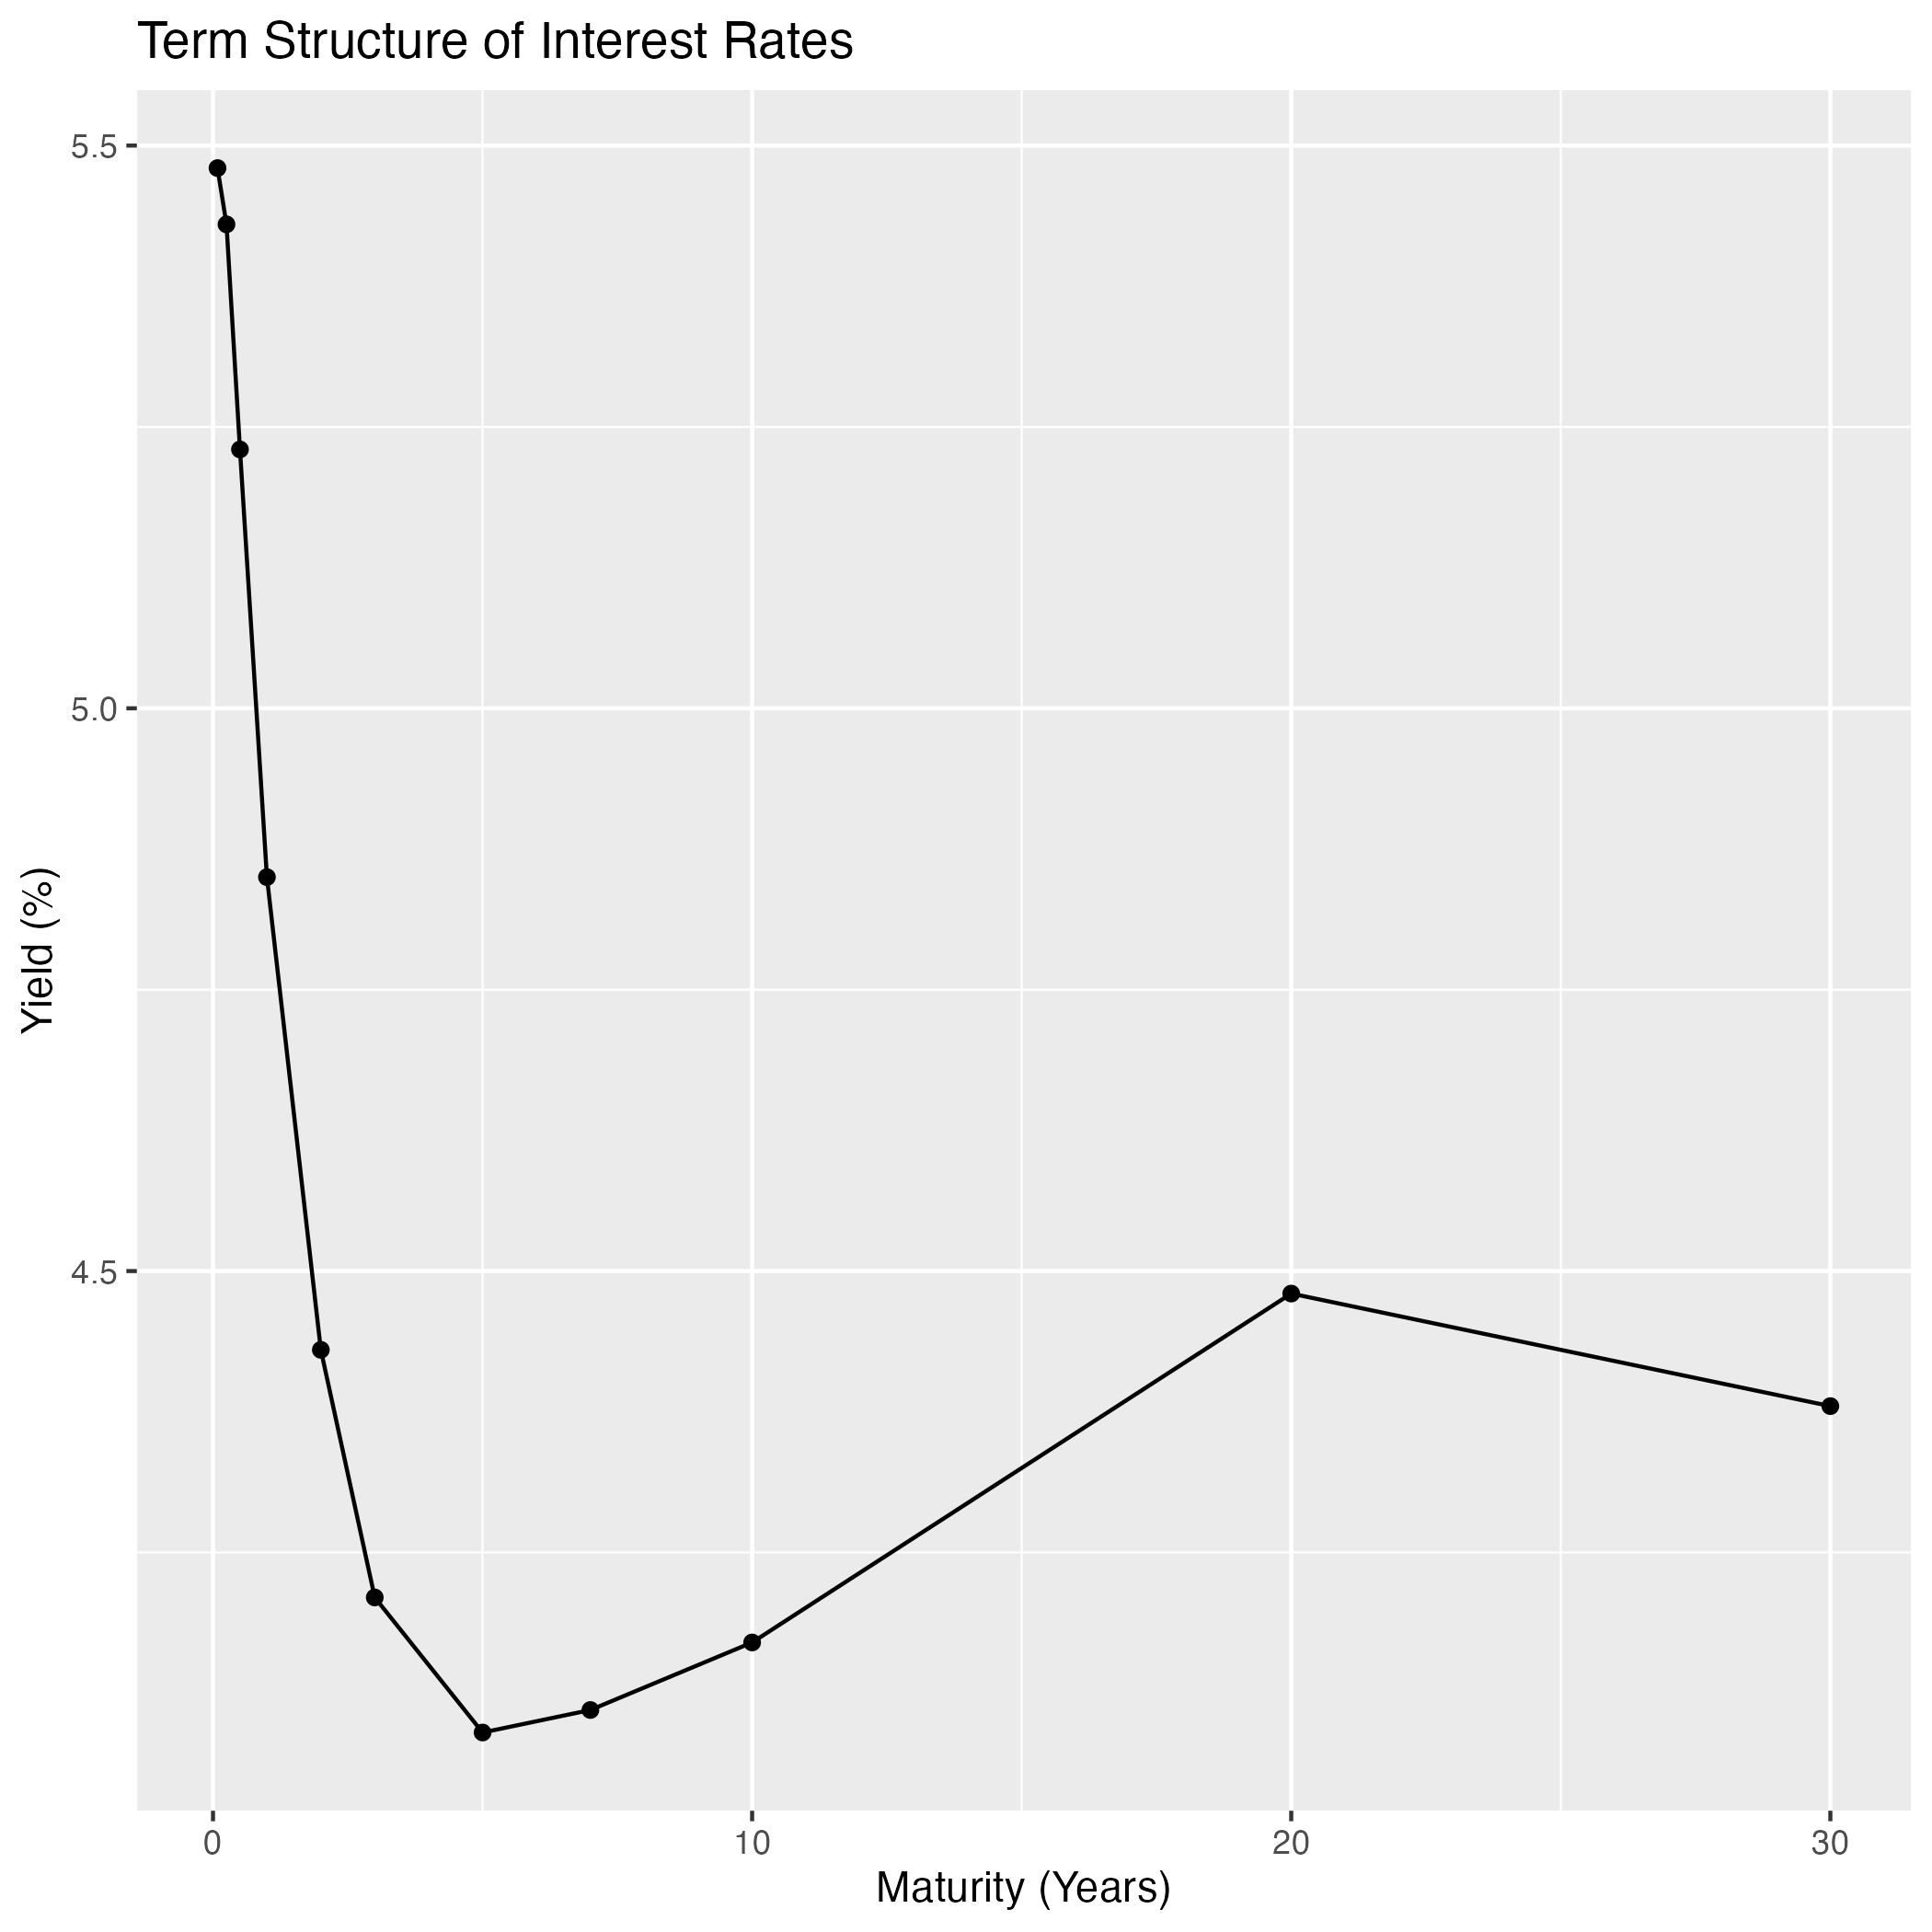
\includegraphics[width=0.8\textwidth]{/Users/cancel/Personal/Coursework/Econ425/HW7/R/YieldCurve.png}
    \caption{Term Structure of Interest Rates}
\label{fig:yieldcurve}
\end{figure}

\noindent\rule{\linewidth}{0.5pt}

\subsection{Equation Explanation}
\[ \sum_{j=0}^{365} i_{1d}^{s+j \times 1d} = 365 \times i_{1y}^{s} - \phi_{1d,1y} \]

This equation expresses the relationship between short-term daily interest rates and the one-year interest rate, accounting for a term premium \(\phi_{1d,1y}\). It approximates the annual interest rate by summing daily rates over a year, considering the compounding effect and term premium. The term premium is included because over long periods, there is uncertainty about inflation and other risks such as default risks.

\noindent\rule{\linewidth}{0.5pt}

\subsection{Empirical Rates in the US}
In the US, \(i_M\) is the Federal Funds Rate, and \(i_R\) is the Interest Rate on Reserve Balances. The Fed directly controls the Interest Rate on Reserve Balances and influences the Federal Funds Rate through open market operations and forward guidance.

\textbf{Why \(i_M \geq i_R\):} This must be the case because if the Federal Funds Rate (\(i_M\)) were lower than the Interest Rate on Reserves (\(i_R\)), banks would prefer holding excess reserves over lending in the interbank market, leading to a liquidity shortage and driving up the Federal Funds Rate until equilibrium is restored.

\noindent\rule{\linewidth}{0.5pt}

\subsection{Control of Empirical Rates}
\begin{enumerate}
    \item \textbf{Federal Funds Effective Rate:} Indirectly controlled by the Fed through open market operations.
    \item \textbf{Interest Rate on Reserve Balances:} Directly controlled by the Fed.
    \item \textbf{Overnight Reserve Repurchase Agreements Award Rate:} Indirectly influenced by the Fed through market operations.
\end{enumerate}

\textbf{Relationship among rates:} Interest Rate on Reserve Balance \(\geq\) Federal Funds Rate \(\geq\) Overnight Reserve Repurchase Agreements Award Rate.

\noindent\rule{\linewidth}{0.5pt}

\subsection{Evaluation of the Claim about Fed's Monetary Policy}
While the Target Range for the Federal Funds Rate is a primary tool, the Fed also uses other instruments like open market operations, the discount rate, and reserve requirements to influence liquidity and interest rates. Therefore, the claim is an oversimplification as the Fed's implementation of monetary policy involves multiple tools to achieve its objectives.

\noindent\rule{\linewidth}{0.5pt}

\subsection{Impact of Fed’s Monetary Policy on the US Economy}
The Fed's monetary policy affects the economy by influencing borrowing costs, consumer and business spending, and inflation expectations. Lower interest rates encourage borrowing and spending, stimulating economic activity, while higher rates can cool an overheated economy and control inflation. The Fed's policies aim to achieve maximum employment, stable prices, and moderate long-term interest rates. Local banks rely on the Fed to remain solvent, which is crucial for a stable economy.

\noindent\rule{\linewidth}{1pt}

\section{The Taylor Rule and Principle}

\subsection{The Taylor Rule}
\[ i_M^t = 2 + \pi_t + \frac{1}{2} (\pi_t - 2) + \frac{1}{2} (y_t - \tau y_t) \]

The Taylor Rule prescribes how a central bank should set the nominal interest rate (\(i_M\)) based on the current inflation rate (\(\pi_t\)), the deviation of inflation from its target (2\%), and the output gap (\(y_t - \tau y_t\)). It provides a systematic framework for monetary policy to stabilize inflation and output.

\noindent\rule{\linewidth}{0.5pt}

\subsection{Comparison with Taylor, 1993}
The given equation aligns with Taylor's original formulation, incorporating both the inflation gap and the output gap. Taylor's 1993 equation emphasized the role of these two variables in setting interest rates to achieve economic stability.

\noindent\rule{\linewidth}{0.5pt}

\subsection{Optimal Behavior of Central Bank}
The Taylor Rule provides a useful benchmark for central banks, offering a systematic approach to setting interest rates based on economic conditions. While not always optimal in every situation, it helps guide monetary policy towards stability by responding predictably to changes in inflation and output.

\noindent\rule{\linewidth}{0.5pt}

\subsection{The Taylor Principle}
The Taylor Principle states that the central bank should raise nominal interest rates by more than one-for-one with increases in inflation to stabilize the economy. This ensures that real interest rates rise when inflation increases, helping to control inflationary pressures.

\noindent\rule{\linewidth}{0.5pt}

\subsection{Dynamics of Inflation}
When the Taylor Principle holds, increases in inflation lead to higher real interest rates, which cool economic activity and bring inflation down. Conversely, if the principle does not hold, rising inflation may not be countered effectively, leading to runaway inflation. Graphically, the adherence to the Taylor Principle shows a stabilizing feedback loop, while its absence shows a destabilizing spiral.
\clearpage
\begin{figure}[ht!]
    \centering
    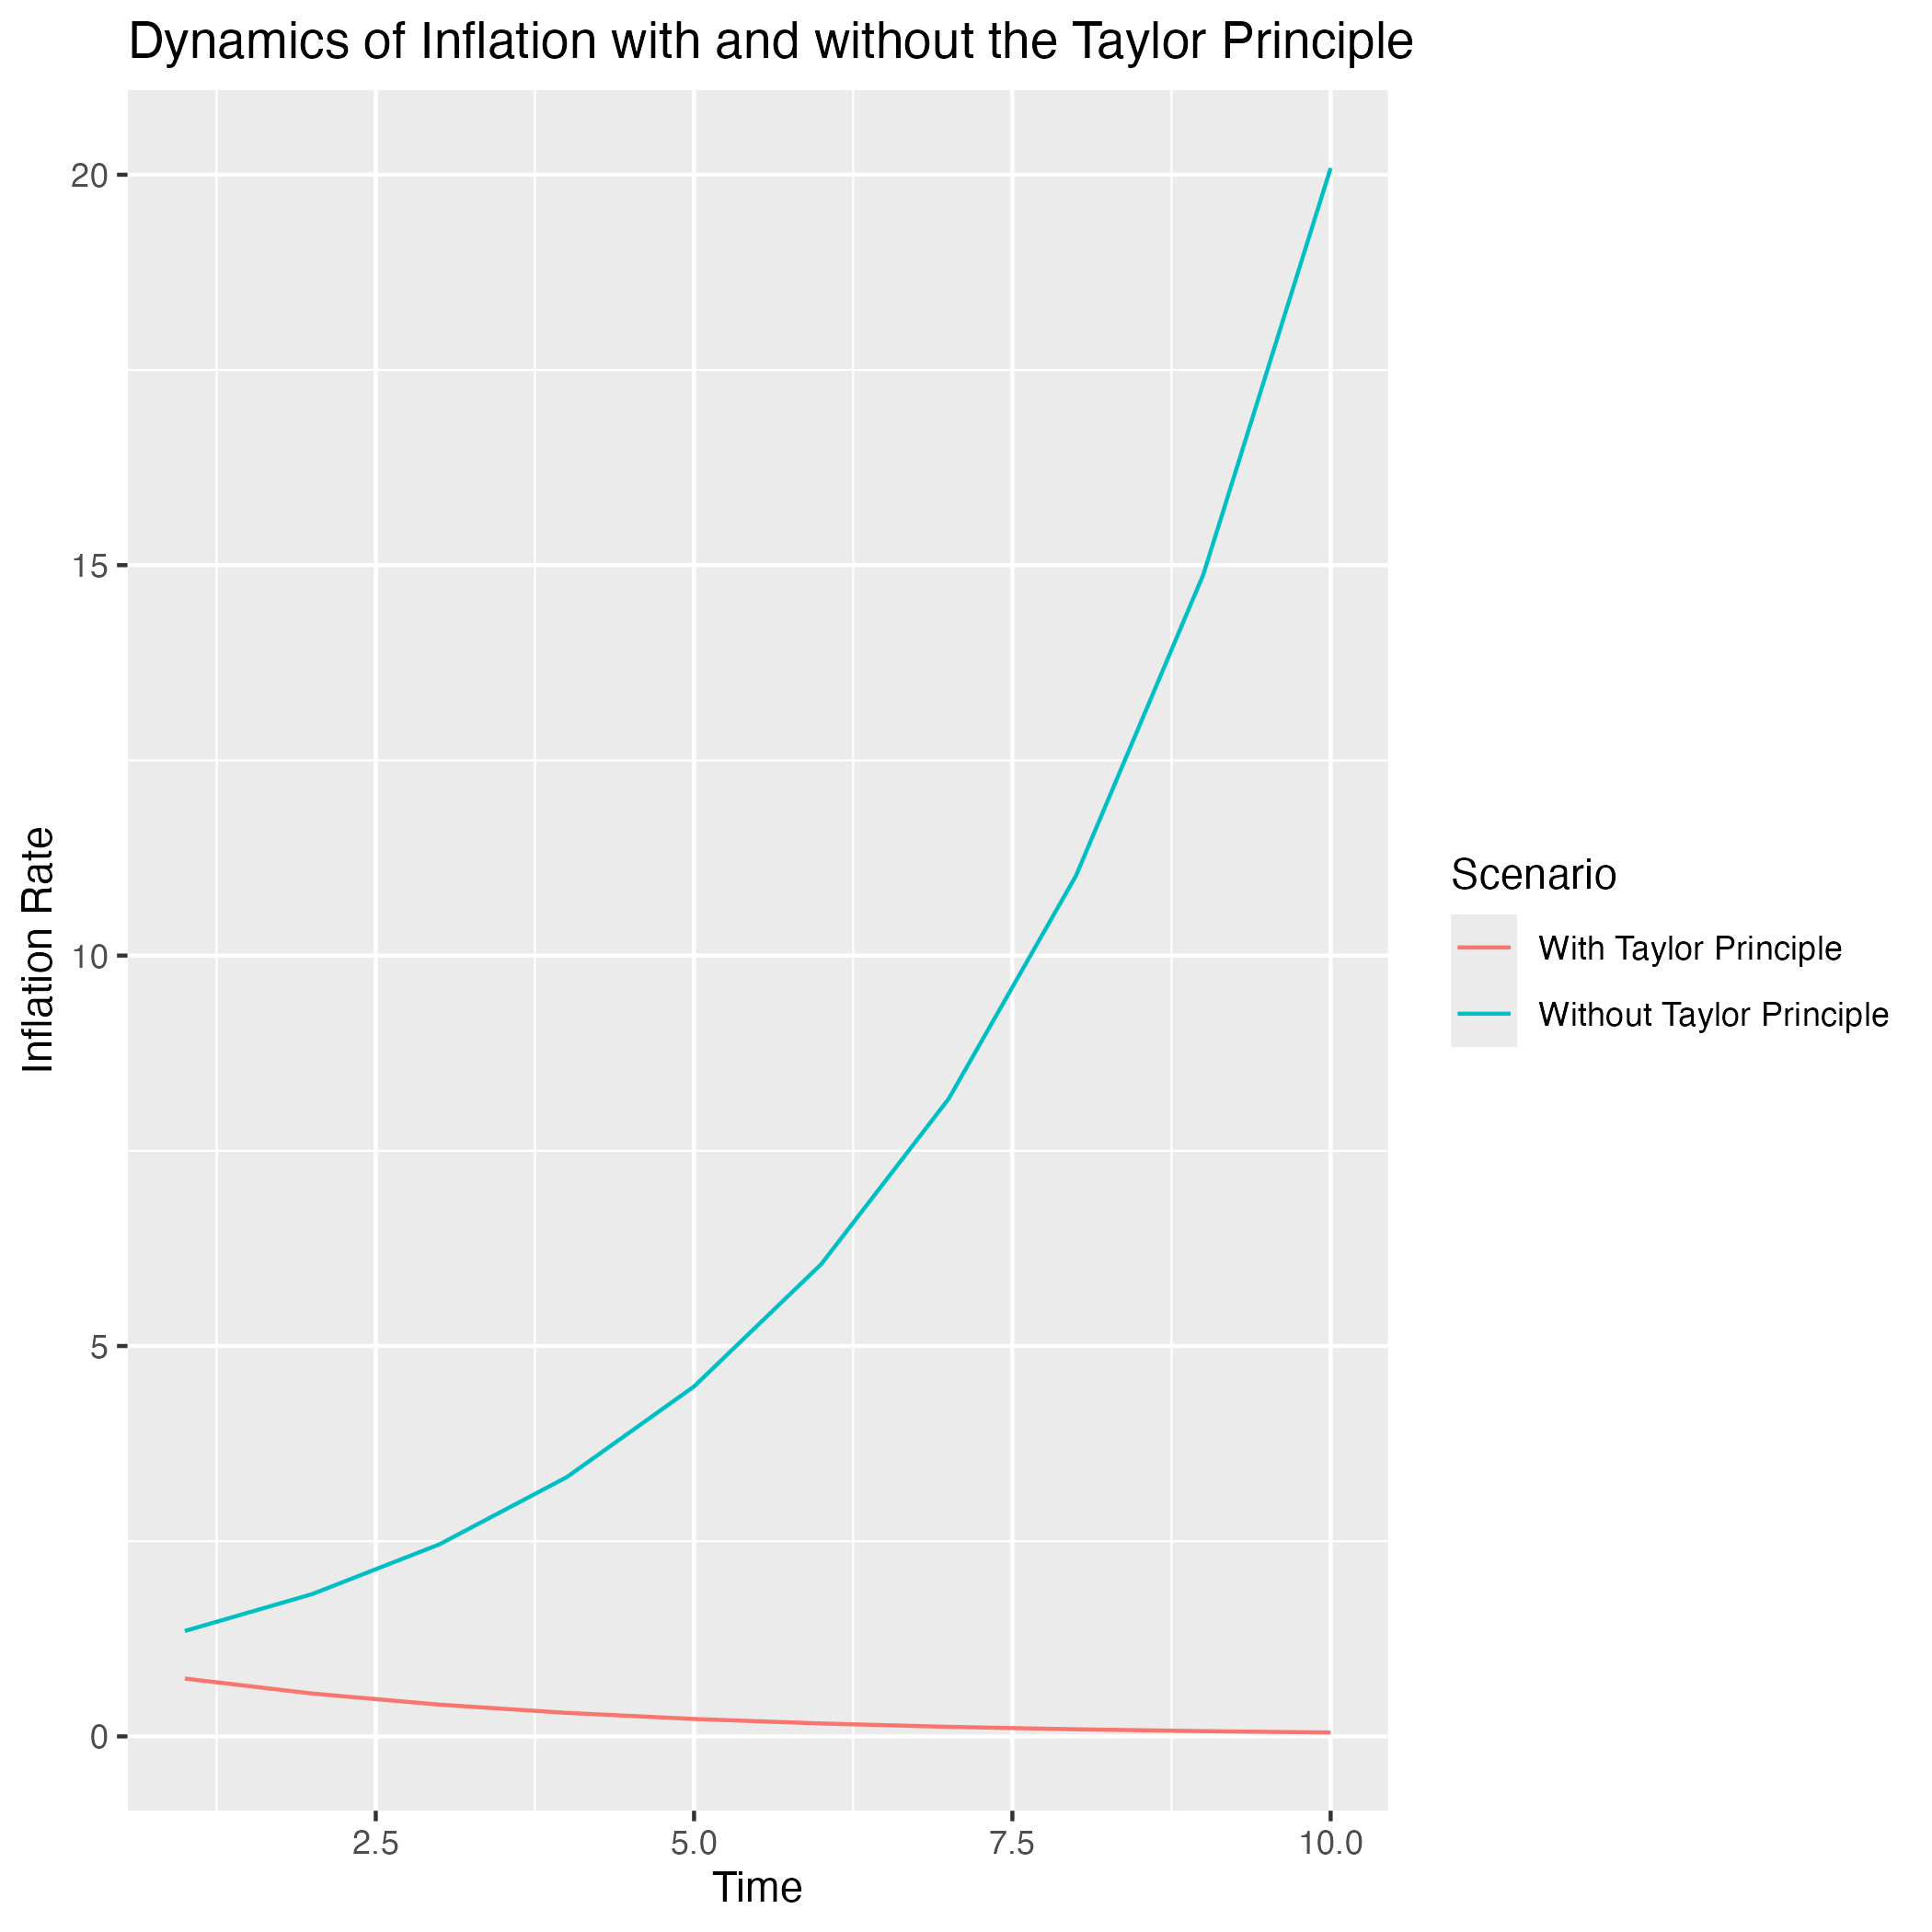
\includegraphics[width=0.8\textwidth]{/Users/cancel/Personal/Coursework/Econ425/HW7/R/InflationDynamics.png}
    \caption{Dynamics of Inflation with and without the Taylor Principle}
\label{fig:inflationdynamics}
\end{figure}

\noindent\rule{\linewidth}{1pt}
\clearpage
\section*{References}
\begin{enumerate}
    \item Federal Reserve Board.\ (n.d.).\ \textit{Board Members}. Retrieved from \url{https://www.federalreserve.gov/aboutthefed/bios/board/default.htm}
    \item Federal Reserve History.\ (n.d.).\ \textit{Current Fed Leaders}. Retrieved from \url{https://www.federalreservehistory.org/people/current-fed-leaders}
    \item Investopedia.\ (n.d.).\ \textit{Federal Open Market Committee (FOMC): What It Is and Does}. Retrieved from \url{https://www.investopedia.com/terms/f/fomc.asp}
    \item Romer, D. (2018).\ \textit{Advanced Macroeconomics}. McGraw-Hill Education.
    \item Challe, E. (2019).\ \textit{Macroeconomic Fluctuations and Policies}. MIT Press.
\end{enumerate}

\end{document}
